\chapter{Methods}
\label{chapter2}

\section{Version Control}
All of the code developed for this project has been managed by git and pushed to a GitHub respository with can be accessed by the link:

\begin{center}
    https://GitHub.com/Anthony-Moran/Final-Year-Project
\end{center}

The history will show the various stages of this project and how we started off with a blank workspace and ended up with this product now.

When implementing the online features, the commit messages became less detailed because the changes were extremely minor (usually one line or printing variables to the console) and changes were being made rapidly for debugging. This was required because the tools that we have used to deploy the app require the changes to be committed in order to come into effect. This differs from the earlier commits where the solution could first be tested locally and then committed only when the changes were implemeted correctly.

% This part might not be necessary
% During this time, a new branch was created in order to isolate the changes, and ensure that there was a stable version of the app as a backup. Since then, the online version has been tested (more details in Chapter 3) and now works, so a pull request was made and now the online is a part of the stable build. A lot of the changes from this pull request actually happen outside of git itself. This includes setting up a server for the web app as well as configuring a service to host the websocket server. This configuration did include two new files that can be seen in the pull request, which is the Procfile as well as a requirements.txt file, which were necessary to make the websocket server work. Finally, the last major change was made to the server (main.py file) and this was so the backend could function correctly with the websocker server provider. However it should be noted that this change does not overwrite the offline version of the program, which can still be accessed by running the server on a user's devive (other users who wish to join must be on the same network due to the unsecure communication, more on that later).

\section{Back End}

The back end of a web app is often refererred to as the "brains" of the whole operation. This part is responsible for all of the computation, storing of information and is where the server resides. The complement of this is the front end, which receives information from the server and displays the results in a way that is visually pleasing to the end user. These two components are tied together by some form of communication, and there are multiple ways this can be achieved.

The decision for how to distribute computation between server and client can be made by considering multiple factors. For example, computationally high tasks (like cloud gaming) are better suited to the back end because dedicated hardware can process information faster than the average computer or mobile device. However this speed can be capped by the user's bandwidth, which describes the volume of data they can receive over a given time, for example 80Mbps, or 80 megabits per second. Therefore if a calculation can be performed on the client side, that should be preferred so we can cut out the communication entirely. Now the app we are developing is not computationally expensive, so we should process data on the client side right? While this would work, it may not be the best solution for this probem because it would mean duplicating data, for the two players in the game and potentially other spectators. This is common in distirbuted system design and it certainly works but in this case it would be better to store all information on the server so that there is a single point of truth. This ensures that all participants are synced and if the client needs information, the server is responsible for sending it.

\subsection{Python Server}

During early testing, a simple python server was used to load my web app, it can be created using the following command in the terminal:
\begin{center}
    \begin{lstlisting}
        python -m http.server 8000 --bind 0.0.0.0
    \end{lstlisting}
\end{center}
This requires python to be downloaded in order to run. The command creates a server that can be accessed on the \emph{local} network by searching for the device's IP address followed by the port number, which is 8000 in this example. For clarity, the url would be \emph{http://123.4.5.678:8000}, replacing the "123.4.5.678" with the IP address of the device calling the command. Notice that it is only accessible to user's on the same network, this is due to the fact that most home networks are not accessible from the internet. While this is helpful for testing during development, we will need to use something else to make our chess app truly remote.

\subsection{GitHub Pages}

This brings us to GitHub Pages. Using this service, we can host our web app on the internet directly from our online repository. What this means for us is that any time we push our changes, GitHub will redeploy the app automatically. The benefit of using this over another hosting service is the fact that GitHub Pages is built into GitHub and requires no addtional setup. However, if any experimental features are needed to be developed, they can be done so on a new branch and this ensures that only the stable version of the app is accessible online.

The link to the website is: \url{https://anthony-moran.github.io/Final-Year-Project/}

\subsection{Chess Logic}

To implement the chess logic, we are using a python module called \lstinline{chess}. This module contains many helpful classes and functions that we have used to develop our app. We have only used a portion of these features but there is certainly room to expand in the future. In this app, I used the Board class to store the current state of a game. Most interactions with the chess module occur through this class because the server needs to process and send data related to the board; this is specifically important when multiple games are running simultaneously.

The positions of pieces are recorded in a FEN (Forsyth-Edwards Notation) \cite{PGNStandard} string. This method of denoting positions originated in the 19th by David Forsyth and was later adapted by Steven Edwards to make it compatible with chess software. The FEN for the initial board is \textbf{rnbqkbnr/pppppppp/8/8/8/8/PPPPPPPP/RNBQKBNR w KQkq - 0 1}. The first section represents the board; each row is separated by a slash and each letter character represents a chess piece. The numbers represent the number of consecutive blank spaces. The next letter will be either "w" or "b" and denote whether it is white's turn or black's turn respectively. The next four characters denote what castling moves are available and the next section denotes the space behind a pawn that has just moved two spaces or a dash if this is not applicable (this is necessary for an en passant move \cite{EnPassant}). The final two numbers represent the halfmove clock and fullmove number and are used in end game conditions, however we only consider checkmate and stalemate in this app.

Some custom methods were required for the purpose of extracting unique data and/or formatting to make data more consistent for sending. A function that was surprising not to see in the chess module was for the ability to get the legal moves for a given piece. There was however a function that generated all legal moves, so we can wrap it in a new function and then extract only the moves from the space that we are interested in. In terms of data formatting, a client could ask for the name of a piece on a given square and the current chess function would return either a string or the value \lstinline{None}. Therefore we can wrap that in a new function too and return the string if there is a piece there, otherwise we send the empty string.

\subsection{Game Management}
\label{GameManagement}

Current games are stored in volatile memory on the server, this means data is lost when the server shuts down. This app does not store games on a database and for that reason, games should only be played if they are intended to be finished within the same session. A database would be out of scope for this project, especially because it would require adding the ability to create accounts and associating game IDs with user IDs. Instead, the server uses a dictionary (a hash map) to store game keys to a tuple containing a chess.Board object and a set of connected users.

A customised function has been written to generate random game keys. It concatenates a random combination of letters and numbers, and then makes sure the key doesn't already exist before returning the value. For a length of 4 characters, there are $(26 + 10)^4$ possible game keys that can be generated, which is well over 1 million, and should be more than enough for the scale of this project. However the program has been designed, so that changing one constant value, which is clearly labelled \lstinline{JOIN_KEY_LENGTH}, can be changed and increase the total number of available keys as a result. It may be tempting to run an infinite while loop to generate keys until a unique key is found but there is no guarantee that a key will be generated in a reasonable time frame. Therefore it is recommended to run a for loop for a fixed number of times, in this program it is 1000 times. However if no key is found, a runtime error is raised and handled appropriately.

When a game has ended or both users have disconnected, the game is removed from the dictionary.

\section{Communication}

% Asynchronus
% Network speed - applicable to online version

Our server is able to process all of this information but now we need a way for it to send this data to our clients.

\subsection{Flask/FlaskRESTful}

% what research? and why is it less efficient?
The initial solution to this was to use flask and flaskRESTful, making use of the GET and POST requests over our already established http(s) connection. This solution did work but because we are making a game that takes place in real time, therefore the board needs to update everytime a user makes a move. However a http server only sends messages, when requested. Therefore the clients must continuously check the server to see if the opponent has moved. After some research, this is a recognised process, called "polling". This is not very efficient because most requests will not return data and it is a waste of bandwidth. Surely there is a better method of communicating, instead of this request/response model?

\subsection{Websockets}

Websockets are the answer to this question. After discovering this new bi-directional form of communication, there was a helpful guide \cite{Websockets}, which aided in the conversion from http requests to websocket communication. The guide was making connect 4, which differs from chess, so the final solution varies from the finished code in the guide \cite{CompleteCode}. The code uses the same functions as defined in the guide, excluding the replay and watch functions. A replay function was not necessary because we can send the board as a fen string when we need a full representation of the board. And then due to time constraints, the ability to watch a game was not implemented. The business logic inside each function is different for the reasons given prior. However the formatting of the send/receive data shares some similarities. They both send data as a JSON string and include a "type" key that indicates what type of data is being sent. Similar to the server code, the client code follows the same structure, using an \lstinline{init}, \lstinline{receiveHandler} and \lstinline{sendHandler} function, which are all called once the DOM elements have loaded. We have also added an additional event, which detects when a websocket connection is closed and how the event should be handled.

The server establishes a new websocket connection and as we haven't provided an explicit host, "all interfaces are assumed" \cite{NoHost}. We are interested in the websocket connection with address ws://123.4.5.678:8001, assuming we are using the same IP address as the earlier example and listening on port 8001. We quickly notice that this is very similar to the browser address but http is replaced with ws (and using a different port); this is because websockets do not use the hypertext transfer protocol. The websocket protocol grants us the benefit as mentioned earlier, of bi-directional communication, so we no longer have to poll for data. The server will send data as soon as it is available, without a request being necessary. This is also solves another issue with the previous method, as now, when a user makes a move, all users (including the user who has made the move) can receive the update in parallel via a broadcast. Broadcasting is a method of sending data to all recipients at once and is more efficient instead of sending data to each user individually \cite{Broadcast}. This ensures that all connected users will update simultaneously (excluding bandwidth and other networking factors).

It is important however to address the flaws with websockets and this mainly comes down to their short lifetimes, primarily on mobile devices. For mobile users, exiting the browser or locking the device will break the connection, which could happen in a real life scenario for someone using our app. Earlier in this section, there was an addition added, called the connection handler, and this is an instance where it is used. The page will be reloaded with a query string of "reconnecting=true" and will load a page that features a link named "Rejoin" that will send the user back to their game after being pressed. If in between this time, someone else were to join the game with the same key/link, this new user would take their place and the original user would not be able to join. This is a minor problem, and is outside the scope of the project, so it will remain that way. Additionally, during development, it was noticed that refreshing the page with only one player in the game would cause the game to dissapear. This was due to an unforseen consequence of making the game dissapear when both players leave the game. In this niche case, when the alone user refreshes, they temporarily break their websocket connection which causes the server to kill off the game. When the page finishes refreshing and the websocket tries to initialise, the server returns with an error stating that the game no longer exists. To combat this we have added a small amount of buffer time to keep the game alive longer so if someone refreshes the game will continue to exist. Alternatively, if no one joins after the buffer time, the game is erased from memory.

We've handled the main problems of disconnecting from the server but what about the event when the server isn't running and we cannot connect in the first place? It comes back to our connection handler; in the event that the server is not running, the websocket created on the client side immediately closes and this will call the on close event. Initially the close event displays an error message and after some time will redirect the user to the welcome screen. However if a successful connection is established, this functionality is overwritten and a closed socket will instead try to reconnect or will perform other predefined behaviour.

Assuming that we do not run into these issues, the back end and front end will send messages back and fourth until an end condition (in the game) is met, at which stage the connection is safely closed because communication is no longer necessary.

\subsection{Heroku}

The current implementation of websockets only operates on the non-secure websockets protocol and is only accessible to those on the same network, for the same reasons as the http server. Therefore the last step to making our app remote, is to host our server online. \href{https://www.heroku.com}{Heroku} is a cloud platform as a service. This service virtualises its hardware and allows us to use a portion of it to host our websocket server. After some amendments to the code, our clients can now connect to this websocket over wss (websocket secure protocol). In addition to our GitHub Pages website using https (hypertext transfer protocol secure), all of the communication between our clients and server is now encrypted and accessible from the internet.

For the scale of the project, we are using the eco option for our configuration. This will cover what we need, however a feature of this option is that the server will automatically sleep after 30 minutes of inactivity. A user that tries to access the server while it is asleep will have to wait an initial few seconds before the data is received. Future requests are received almost straight away.

\section{Front End}

We have now looked at the data we are interested in and a means of communicating it to our clients. The next step is to develop a friendly interface for our users to interact with our system.

\subsection{The Welcome Page}

\begin{figure}
    \begin{center}
        \fbox{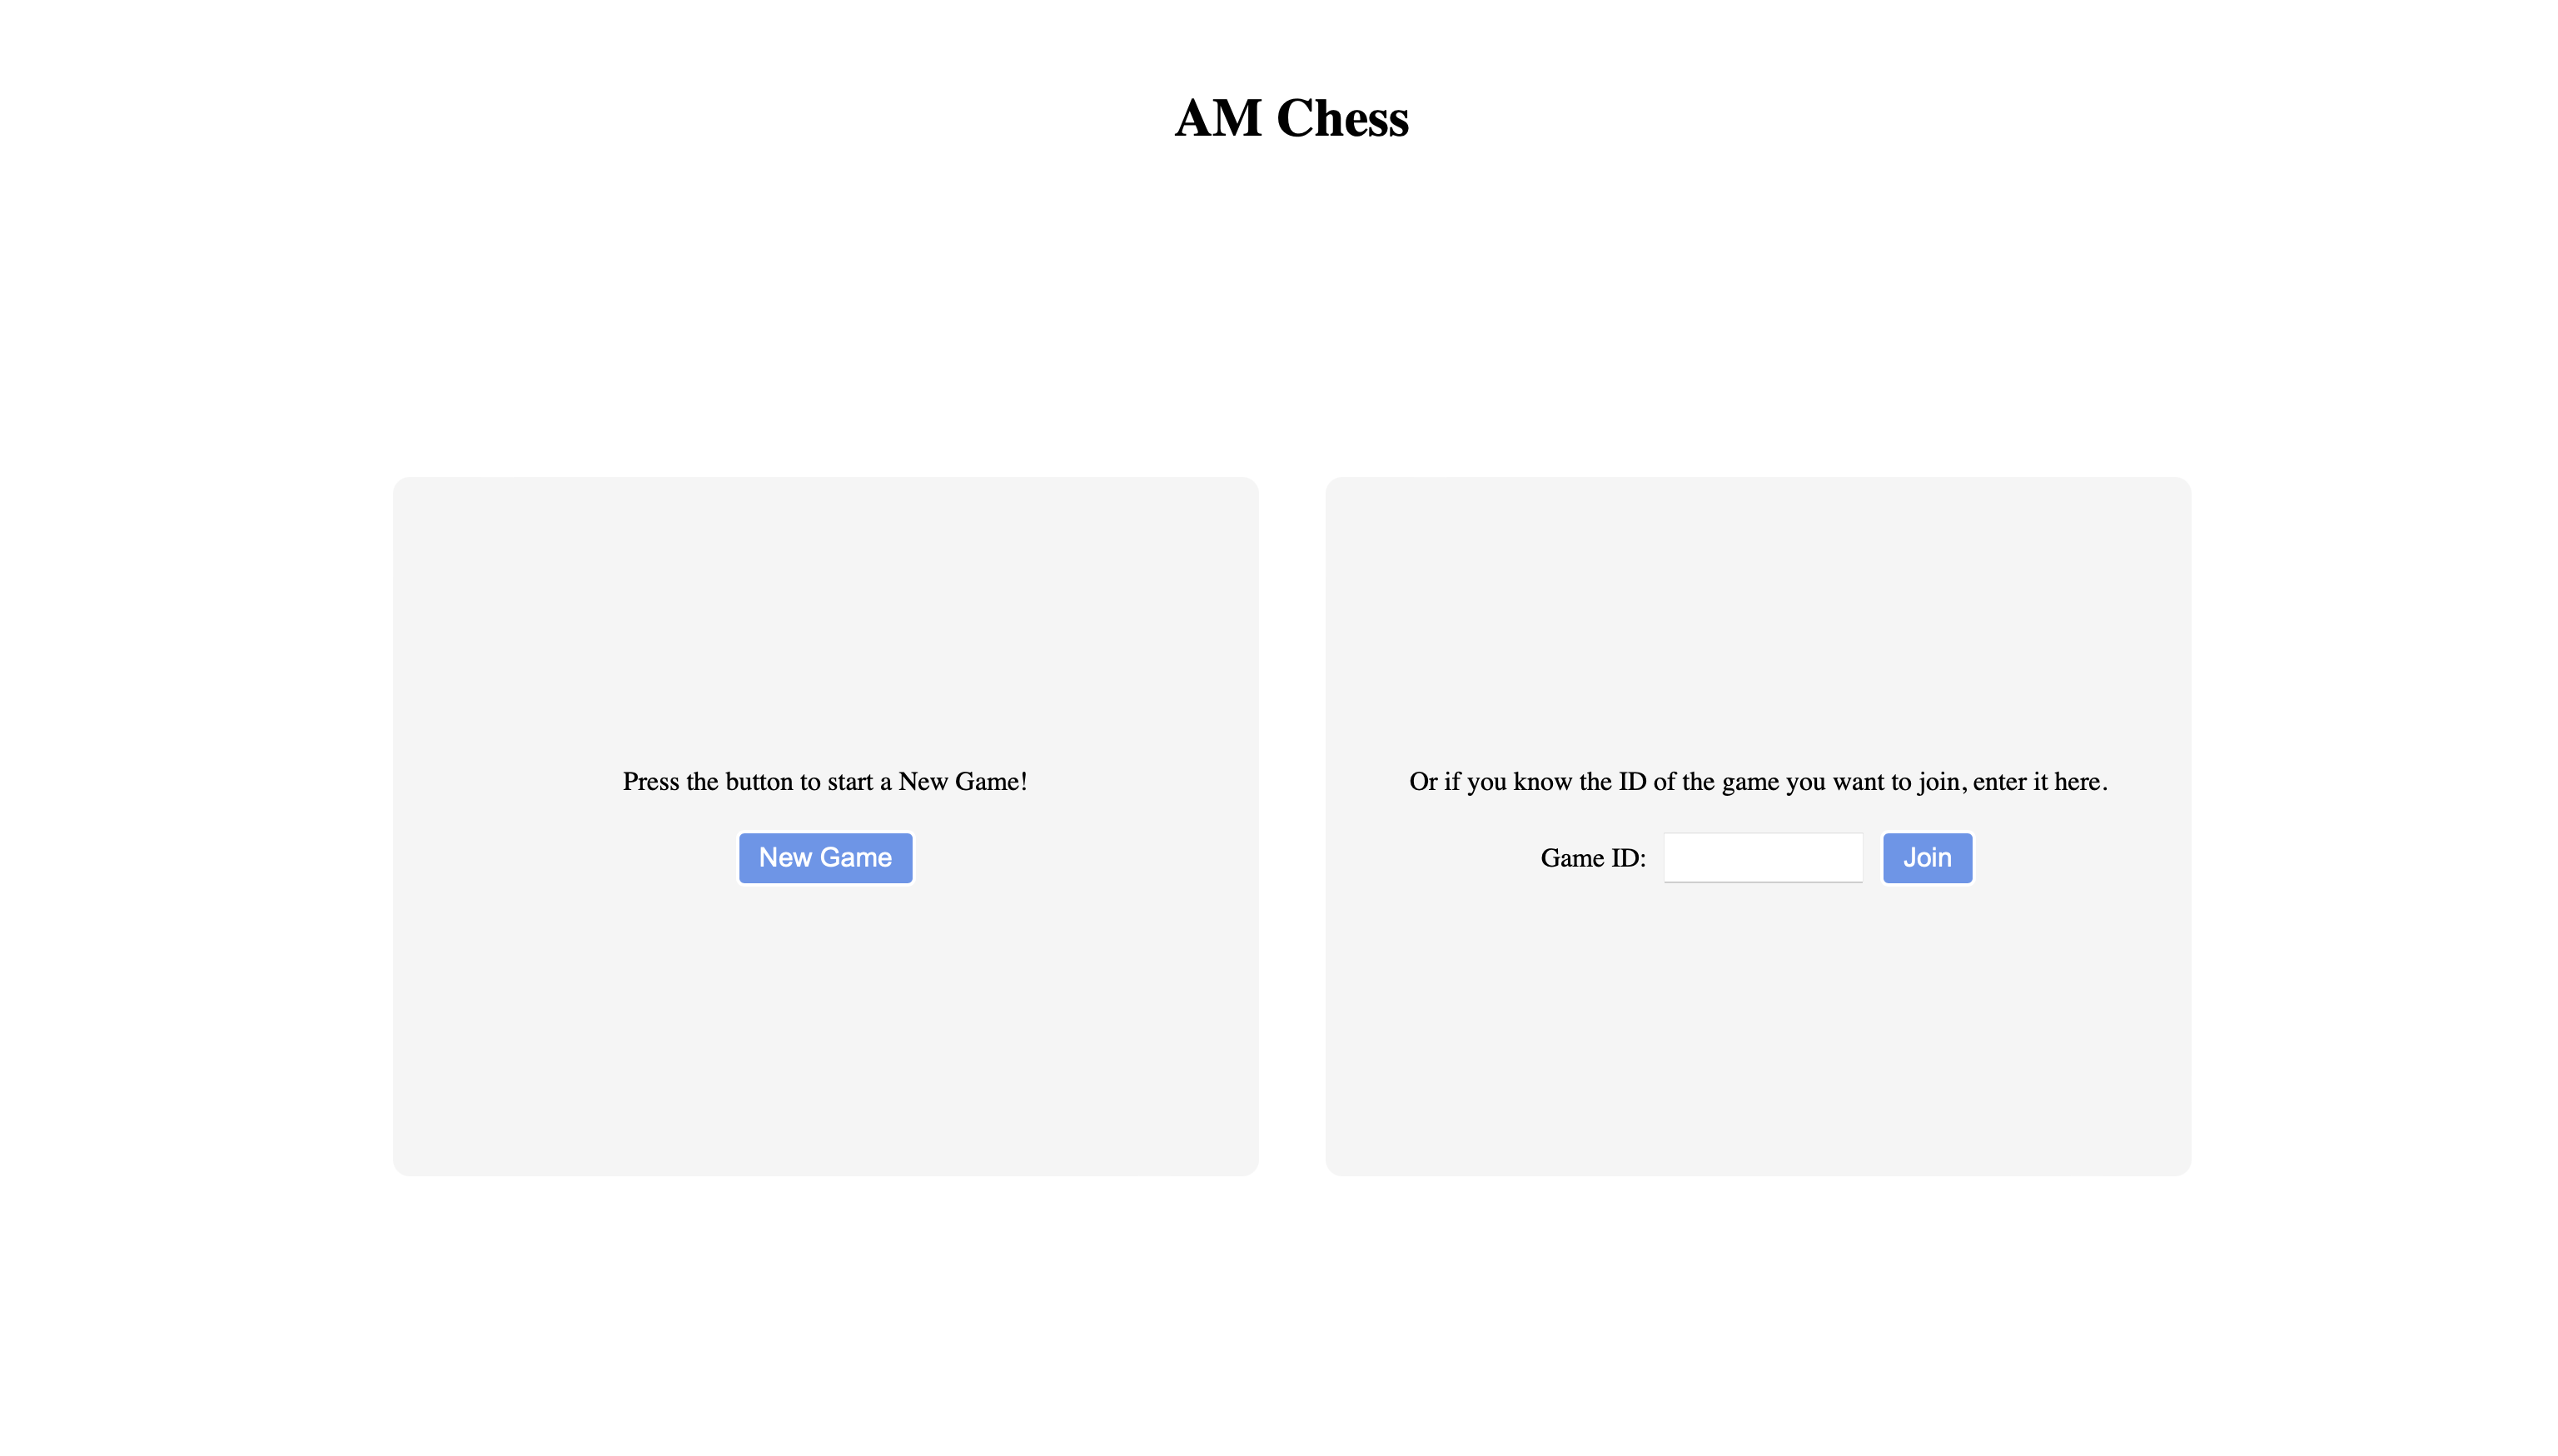
\includegraphics[width=1\textwidth]{welcomePage}}
        \caption{The welcome page of the app as seen on a desktop}
        \label{fig:welcomePage}
    \end{center}
\end{figure}

The welcome page, as seen in figure \ref{fig:welcomePage}, features the title at the top of the screen and then two boxes underneath, with the options for starting or joining a game. The interface is minimal and this design makes it easier for users to digest what they are looking at and make an informed decision for how they would like to proceed. For most users, they will select the new game link, which points to the chess.html file and queries it for a new board. As mentioned earlier in \ref{GameManagement}, there is a possibility that a board cannot be generated. In the unlikely event that this occurs, the server will send an error message, which the browser will alert to the user, using the in-built alert function, and they will be requested to try again. Alternatively, a user may want to join an existing game, in which case they should shift their attention to the second box, to see a textbox where they can enter a join key. If a user enters a non-existing key, the server will redirect them to the welcome page with a query parameter of "badRequest". If this parameter is used, the welcome page will add red text underneath the textbox to alert the user that the key does not exist. This is necessary for users who mistyped the code. The text is red specifically because it stands out from the other colours on the page and is typically associated with erroneous messages.

\subsection{The Chess Page}

The chess page is more complex than the previous page so we will break down its components from top to bottom.

\begin{figure}
    \begin{center}
        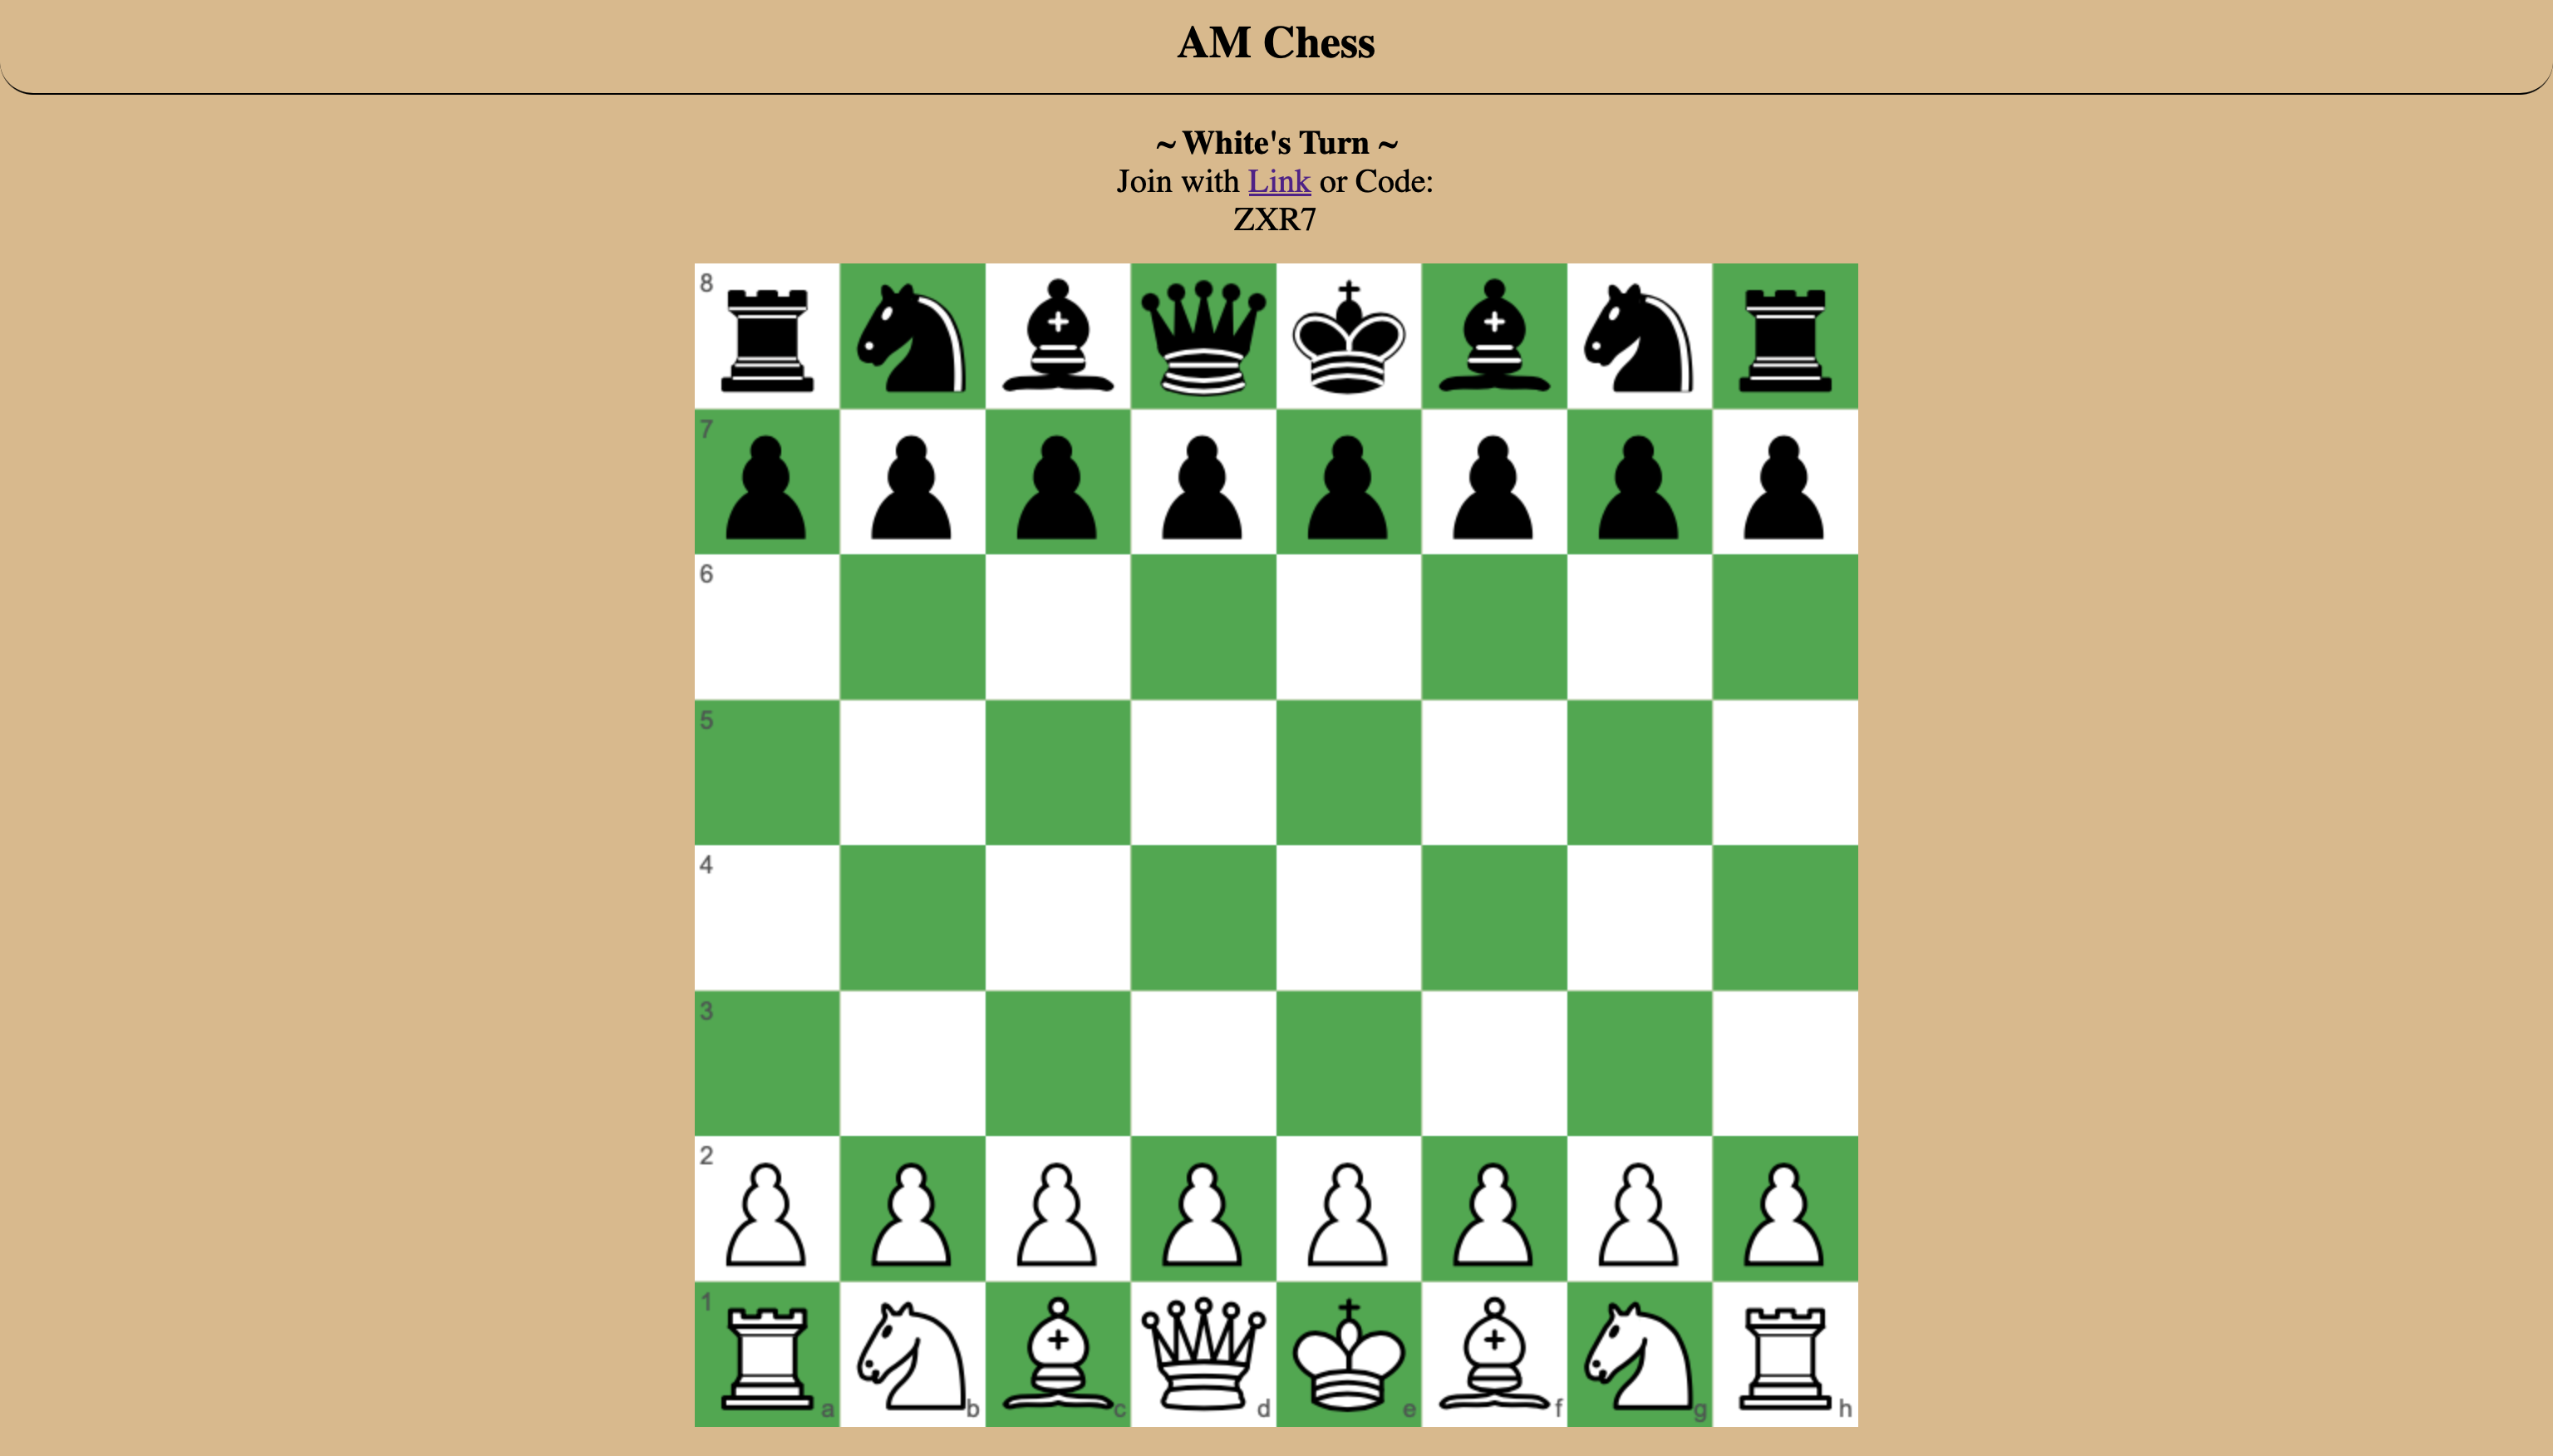
\includegraphics[width=1\textwidth]{chessPage}
        \caption{The chess page of the app as seen on a desktop}
    \end{center}
\end{figure}

We start with the navigation bar. In its current condition it only has one element which is the title of the game, and it acts as a way for users to navigate back to the welcome page. However, if the program were to expand, the design can accomdate for other options, but more on this in \ref{futureDevelopment}.

Secondly, we have the text box. This is a div in the html file that stores all text a user might need to see. This includes the game link, game code and the current player's turn. In addition to the player's turn, it will also indicate if the user is in check. During development, it would sometimes look like the programm was incorrectly not allowing certain moves to be played, when in reality it was because the board was in a state of check. For that reason, it felt necessary to include this in case real user's also faced the same issue. When the game ends, this prompt is replaced by the condition by which the game has ended (i.e. Checkmate or Stalemate) because the information for the current turn is no longer important.

Most importantly, we have the canvas element and this is where we draw our chess board. When the page first loads, the checkered pattern is drawn on the board and once the sprite sheet \cite{SpriteSheet} has loaded, the pieces are then drawn in the positions as provided by the server. For the user that plays as black, the x and y positions of all pieces needed to be flipped to mimic a rotation of 180 degrees. This creates a more immersive experience for the player because it feels like the board is facing them, like it would be in real life.

From this point on, the board is only updated where changes have been made. This was to reduce the volume of computation required between moves, as the majority of the board stays the same. However this didn't come with some setbacks. In general the only spaces that change is the space that the moving piece has come from (which becomes empty) and the space that it is moving to (which will now contain the piece). During developement there were three cases where this rule did not apply, namely castling, en passant and promotion.

% Reposition promotion panel and then insert graphic below
We will start with promotion. This is the act of moving your pawn to the very end of the board, at which point you can choose to "promote" it to another piece (choosing from Queen, Rook, Knight and Bishop). In this case, the new square should instead show the piece selected by the user. The user can select this piece through a menu that we have designed, which features four icons representing the four pieces. Using the mouse or the touch screen, a user can select the piece and the data is sent by the client to the server, to inform it of the decision. The server sends back a generic message that will update the board as expected.

Moving onto the second case, we have en passant. In this case, the piece that we capture (take) is not on the same space that our piece moves to. Before we changed the code, the piece would be removed from the board on the back end but it would look like it is still there on the front end. To fix this, the server sends an additional message after the "play" message to clear the space of the pawn we have just captured.

Finally we have castling, which is the most complex of them all. When the king attempts to castle, we first need to work out the rank and file (row and column) of the rook that the king is castling with and the end position for it. We send the normal "play" message for the king and then a second "play" message for the rook. This had an unforseen consequence of toggling the turn prompt twice on the front end so it would look like the user could move again after castling. This however is only a visual glitch and the server continues to hold the correct turn value on the back end. The reason for this is because the front end toggles the turn to switch between white and black when a user makes their move, which is usually what we want. To resolve this, we can add a flag, called "contribute turn", that alerts the front end whether this move should toggle the turn prompt. This value will default to true because this is the behaviour we would expect in most cases, however when we send the second play for the rook, we will set this flag to false.

We've discussed the special moves but in general these do not occur very often compared to the other moves made in the game. To make a move, the user can select a square with a piece on it using their mouse or touchscreen. This triggers a click event on the canvas and the coordinates of the event are converted to a row and column on the board. The column is calculated from the x value, which can range from 0 to the width of the canvas. We find the column by diving the x value by the size of the squares and rounding down to an integer. The same can be done with the y value to find the row. The chess module stores the squares in a one dimensional array so we need to map the row and column to a single index. The index goes from left to right on board and then down to the next column. This can be mapped by the following:$$index = row * 8 + column$$Once we find the index, we can send this value to the server to indicate that we want to select this square. The square will highlight yellow and available squares will be highlighted blue, as can be seen in figure \ref{exampleMove}. The client is made aware of the available squares because the server sends these after receiving a "select" message. A user can select any blue square to move the piece. If a user attempts to move while it is not their turn they will not be allowed, and the browser will alert them with a message.

\begin{figure}
    \begin{center}
        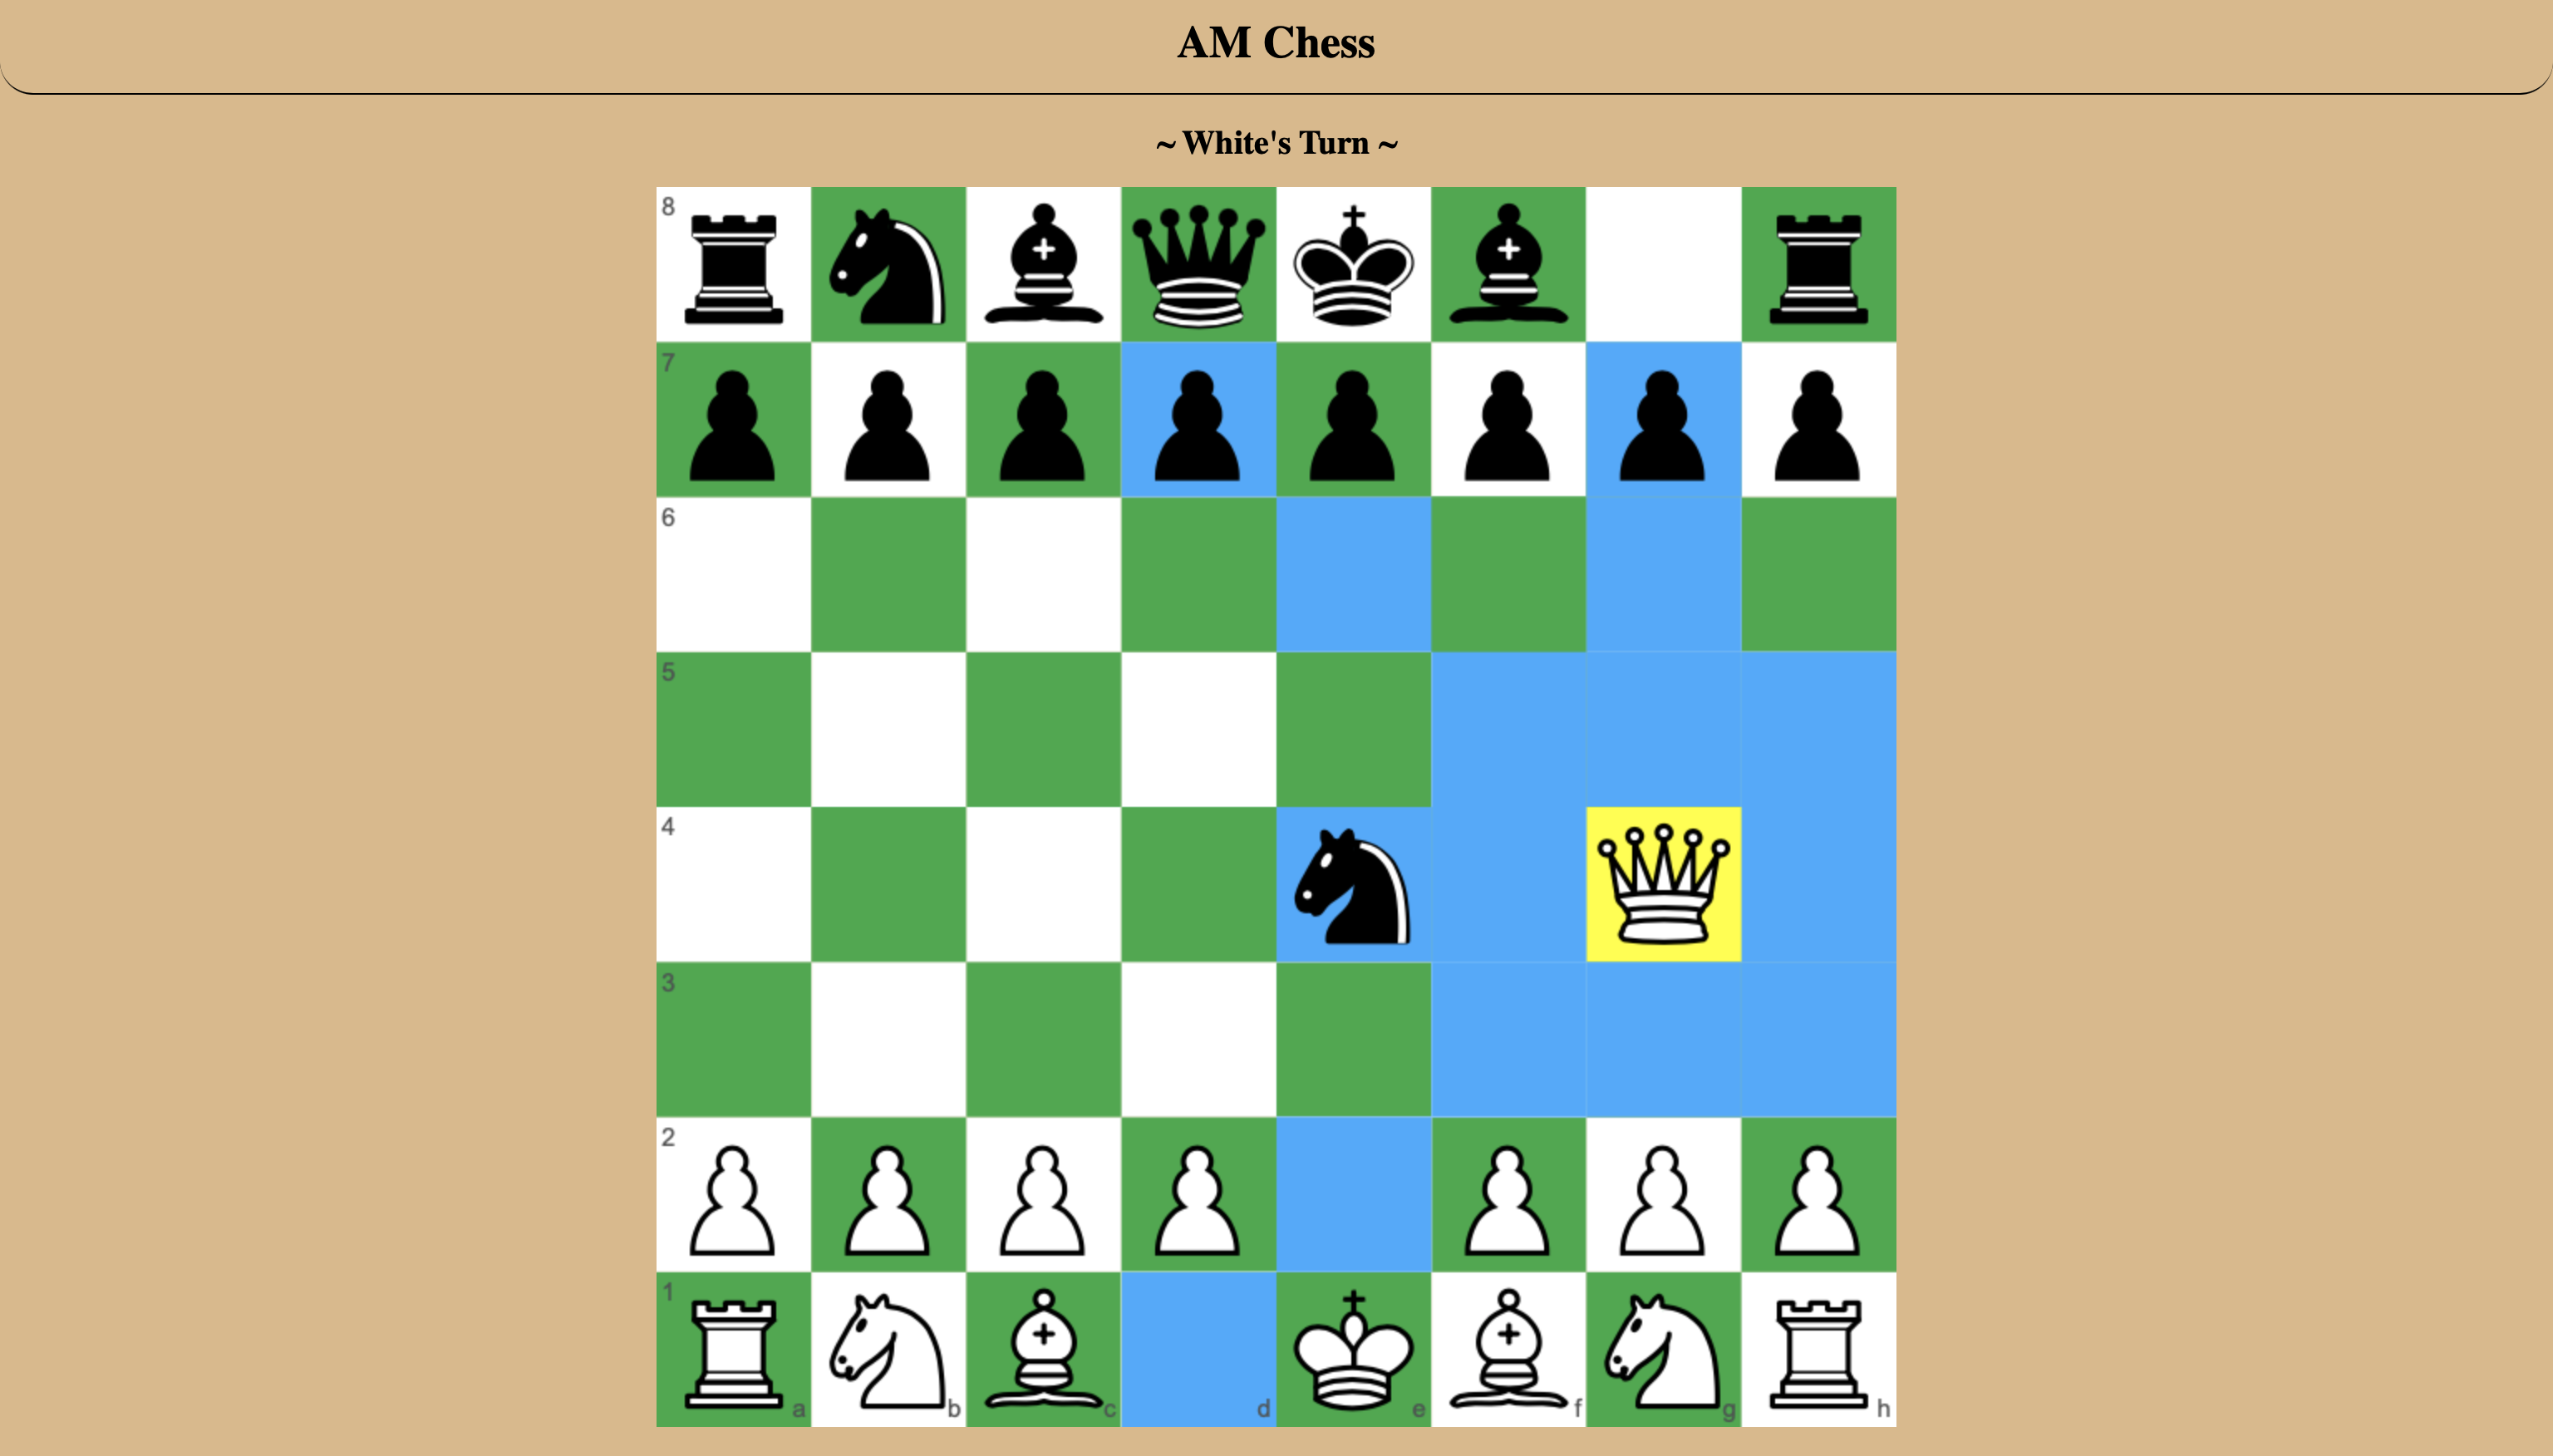
\includegraphics[width=0.45\textwidth]{queenMove}
        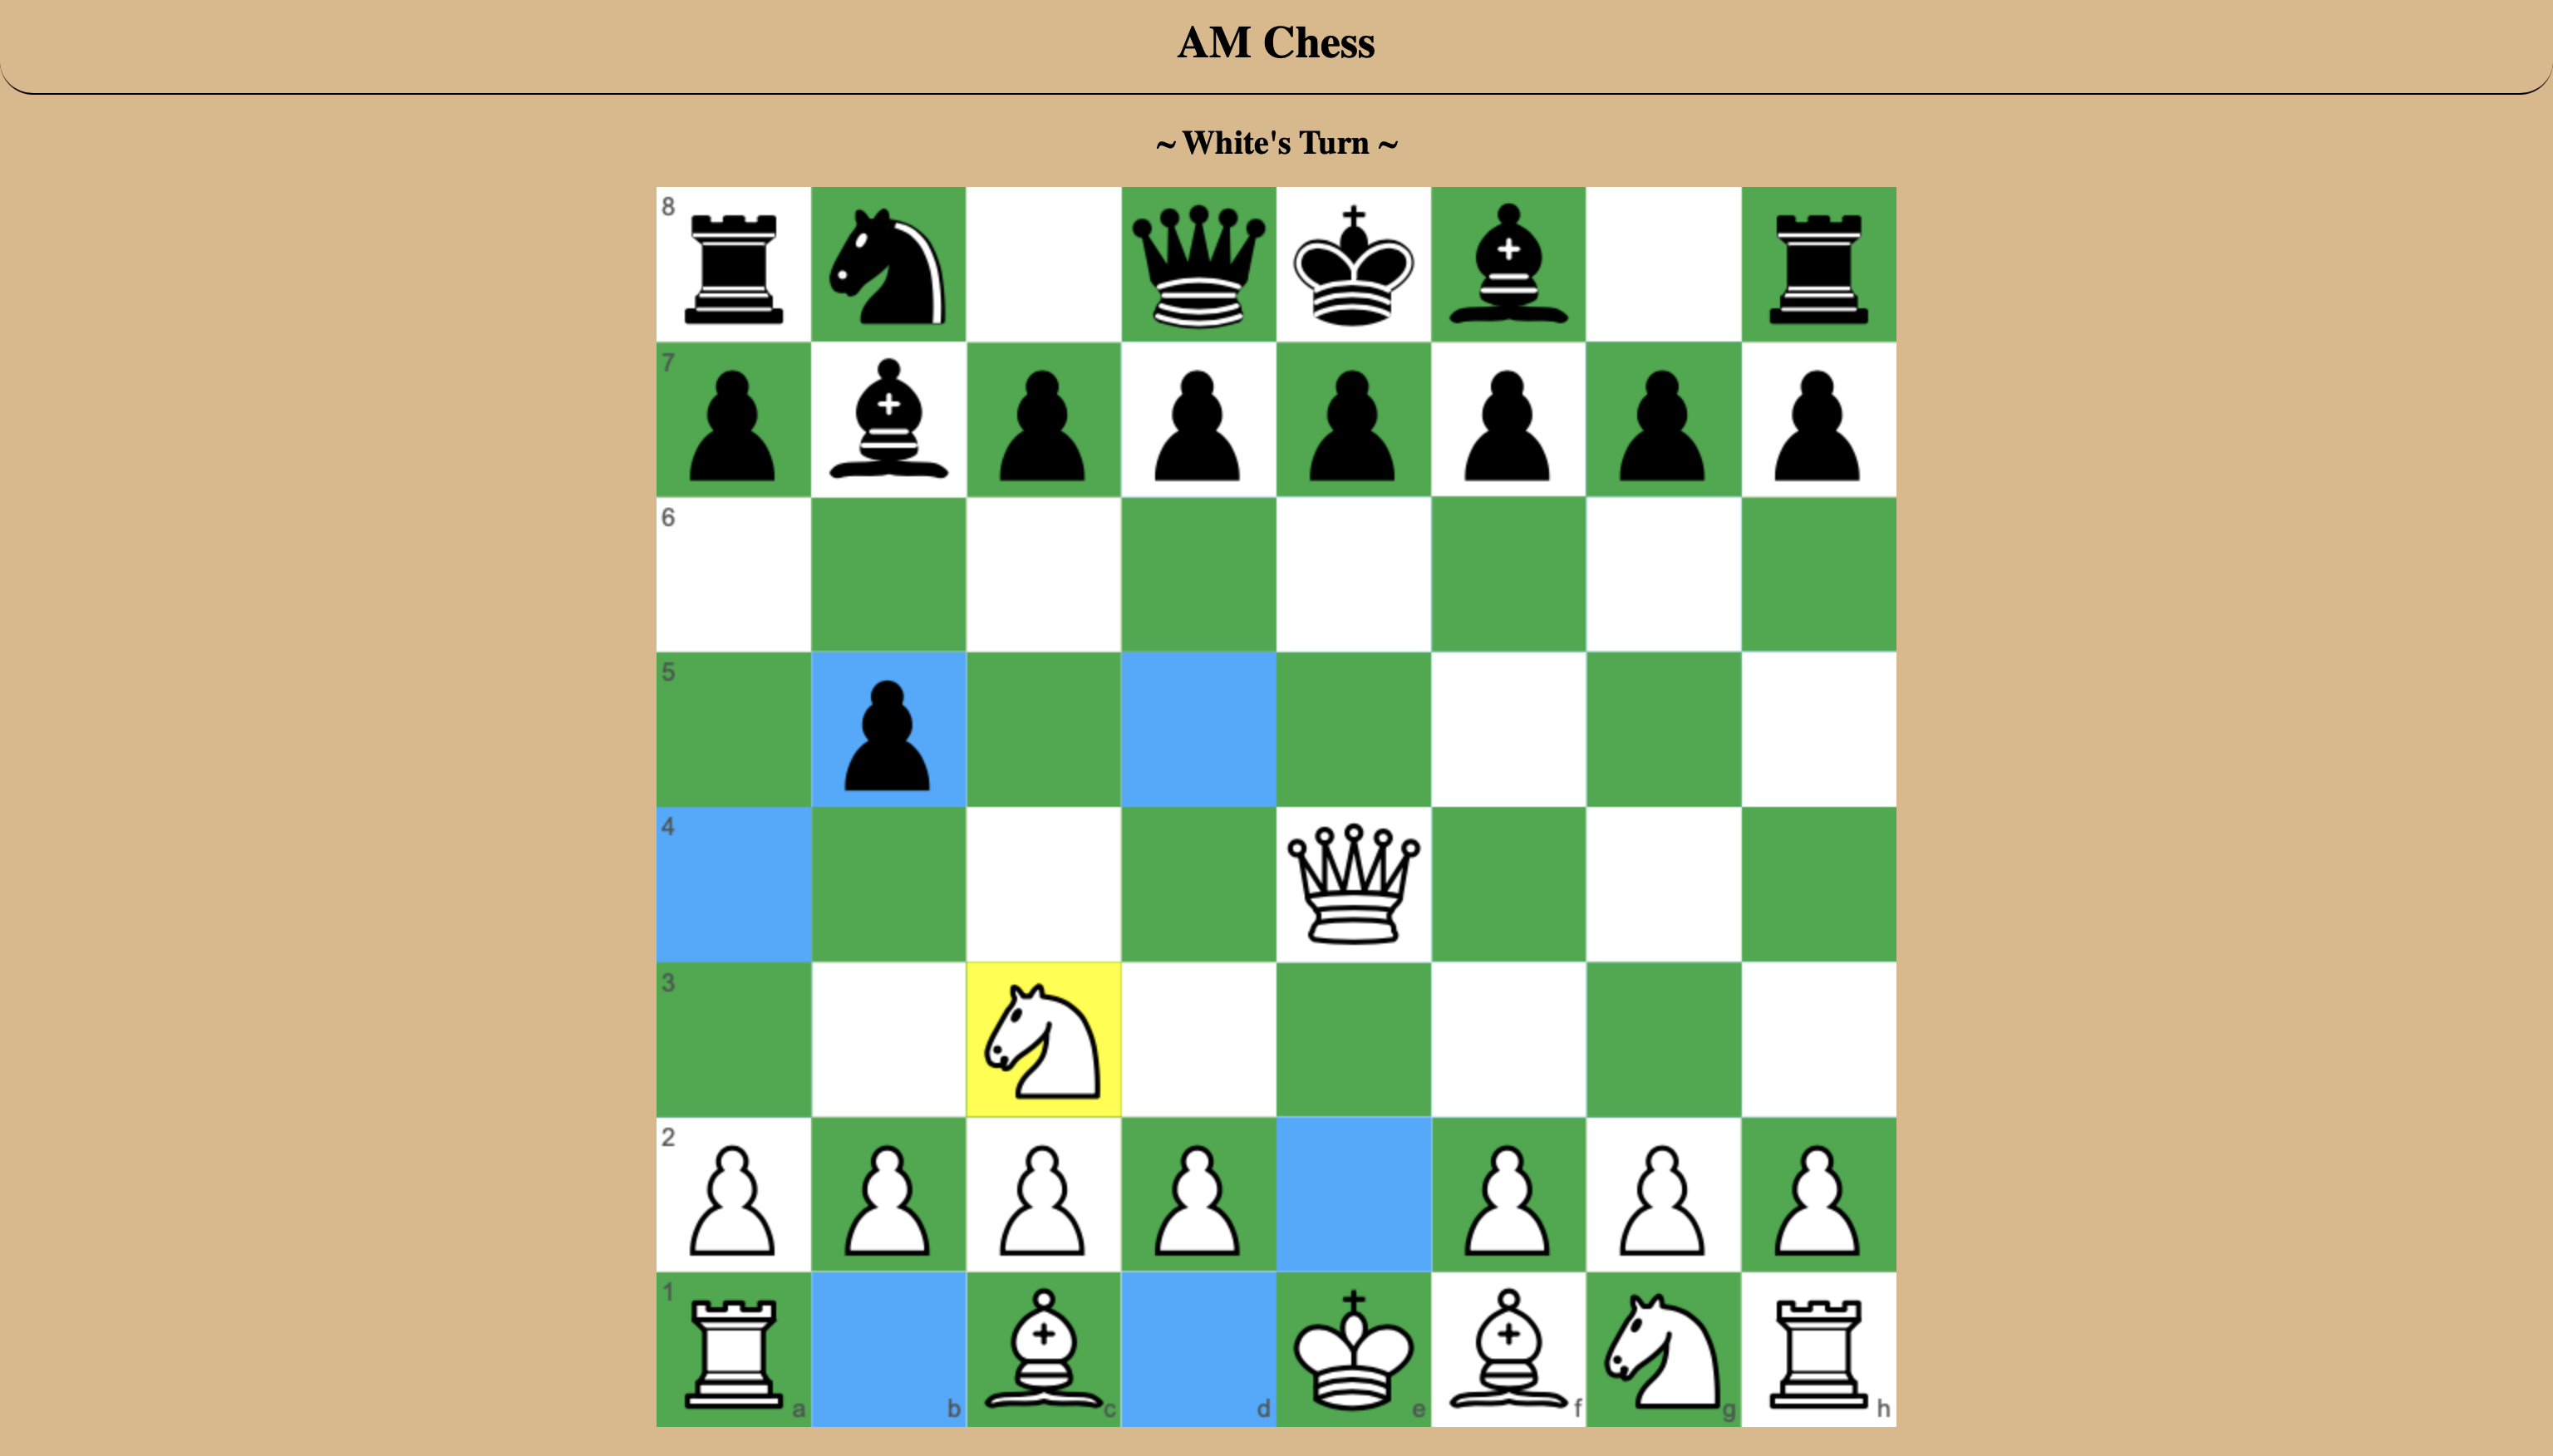
\includegraphics[width=0.45\textwidth]{knightMove}
        \caption{Examples of moving the queen (left) and knight (right)}
        \label{exampleMove}
    \end{center}
\end{figure}

It should be worth mentioning that all of this is only possible if the user has javascript enabled on their browser. The script is responsible for opening a websocket connection and communicating with the server. Without javascript, there is no data to process and the page will be blank.

\subsection{Responsive Design}

% computer users can resize the window and the design adapts: https://web.archive.org/web/20220714020647/https://bencentra.com/code/2015/02/27/optimizing-window-resize.html (debouncing?)

When designing anything on the internet, it's important to remember that users can be accessing resources on any device and when available, the flow of the page should reflect that. Usually this would include css media queries for the size of the screen but this app doesn't contain many elements, so this isn't necessary. We will focus on the orientation of the device because this is what will stop groups of elements from being awkwardly shrunk. We can see in figure \ref{fig:welcomePage} and \ref{fig:responsiveDesign} that the horisontal orientation displays the two boxes next to each other. If we continued this for the vertical orientation, the widths of the boxes would have to squish to fit both of them on the screen. For this reason they are on top and bottom of each other and it also has the benefit of filling otherwise empty space.

\begin{figure}
    \begin{center}
        \captionsetup{justification=centering}

        \fbox{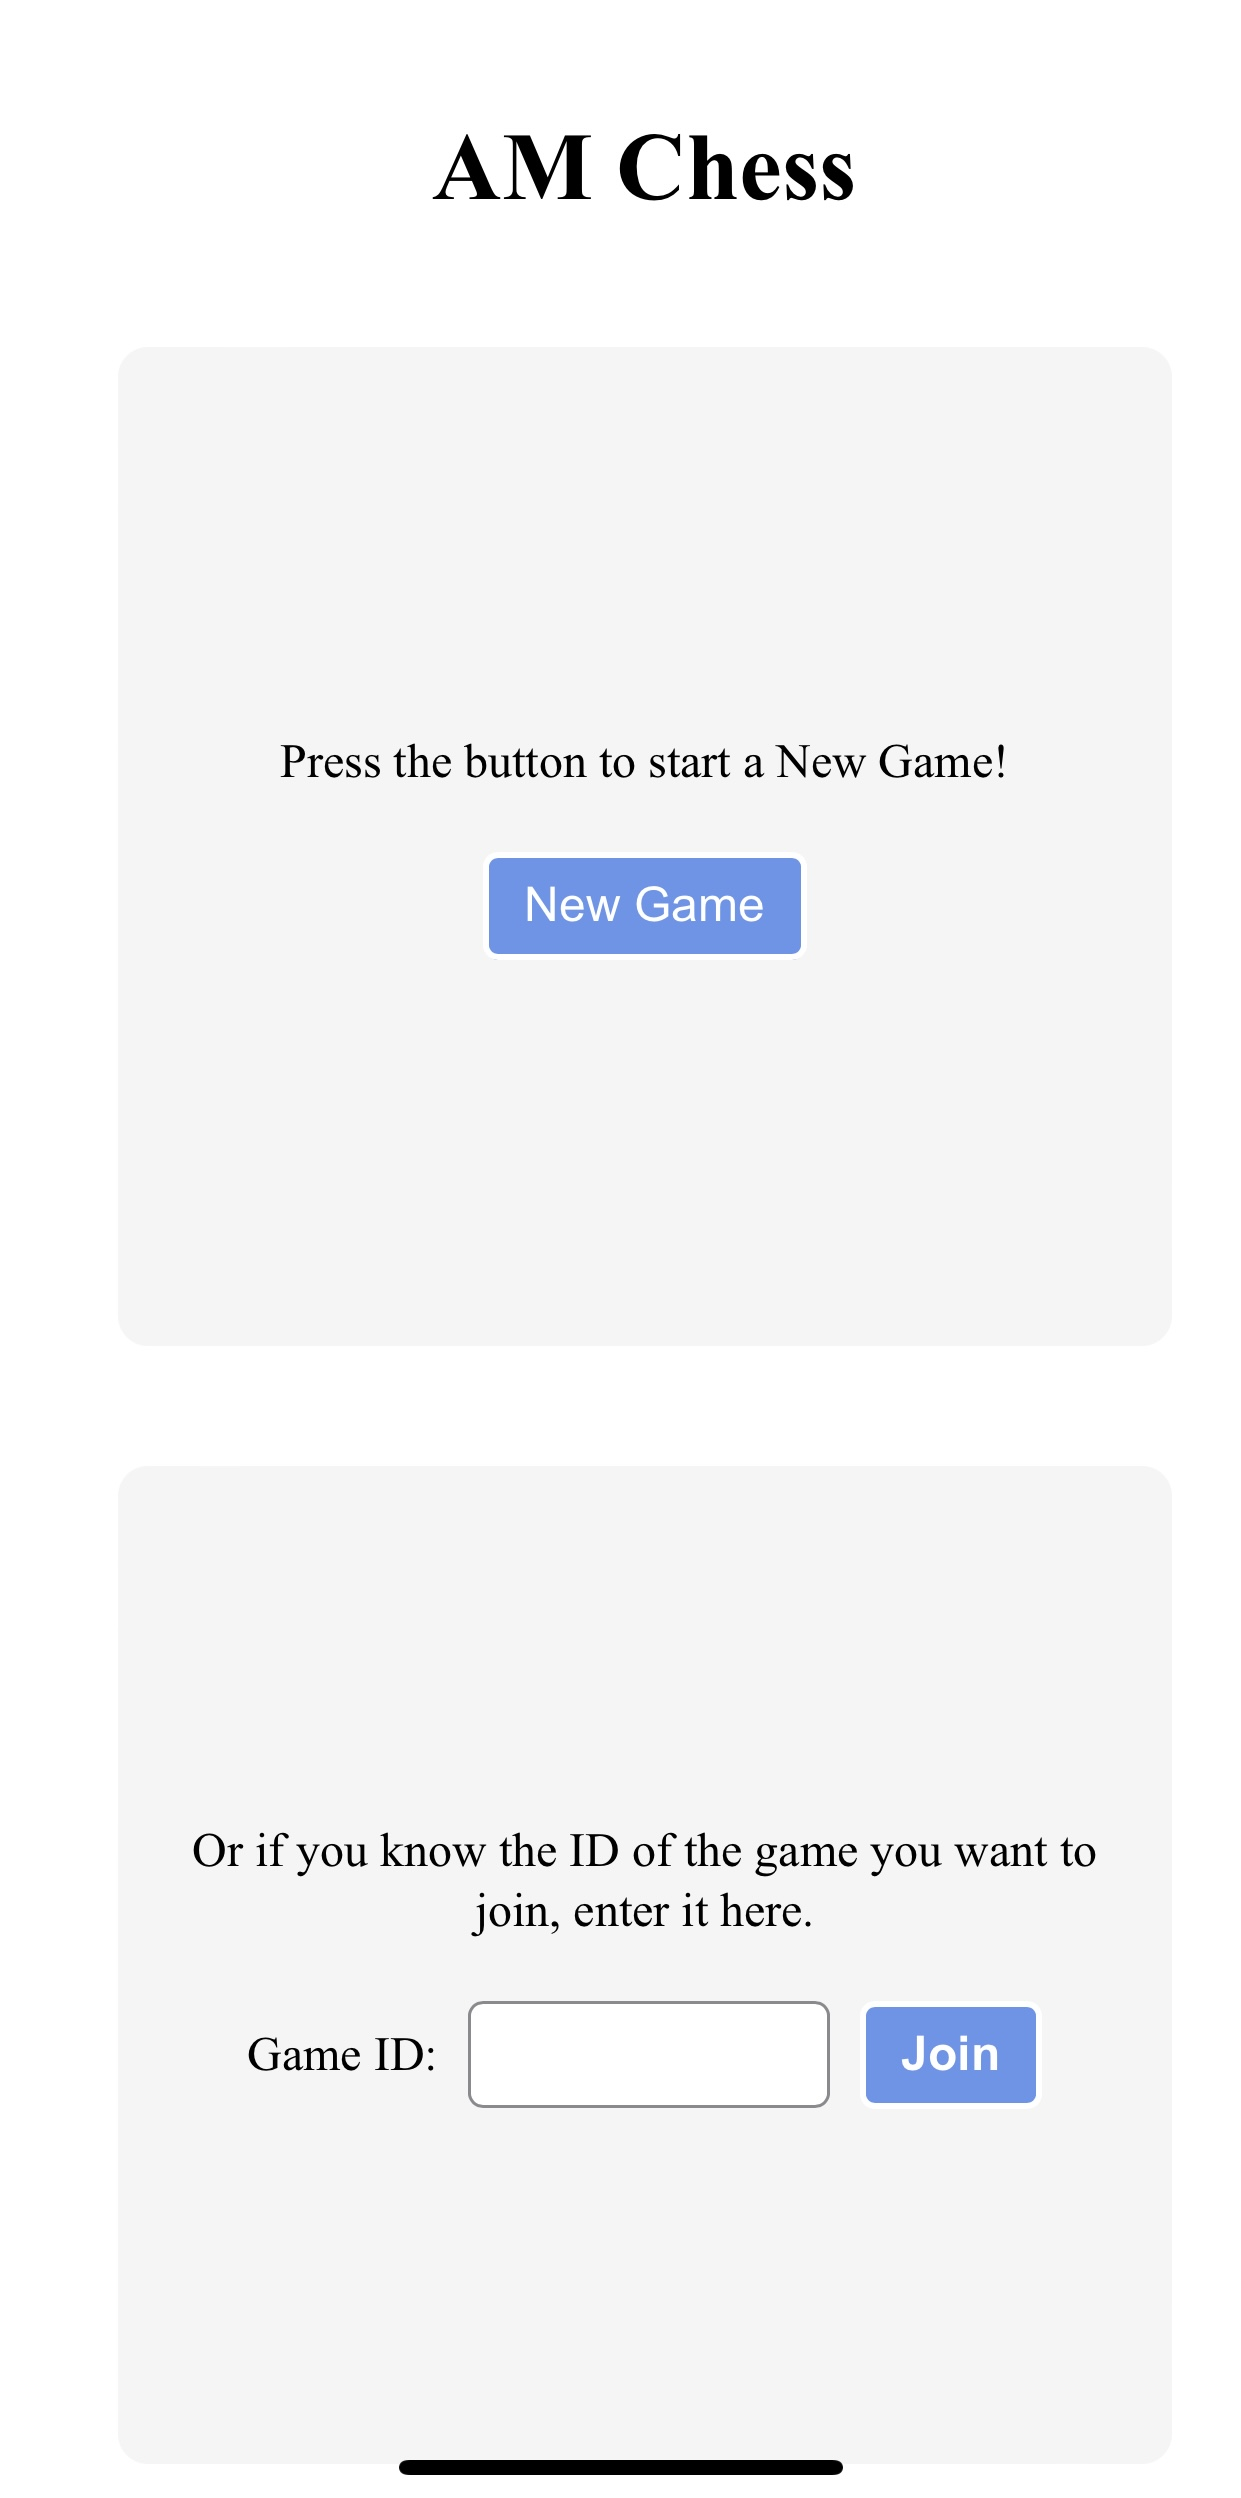
\includegraphics[width=0.25\textwidth]{welcomeVertical}}
        \hspace{1cm}
        \raisebox{0.35\height}{\fbox{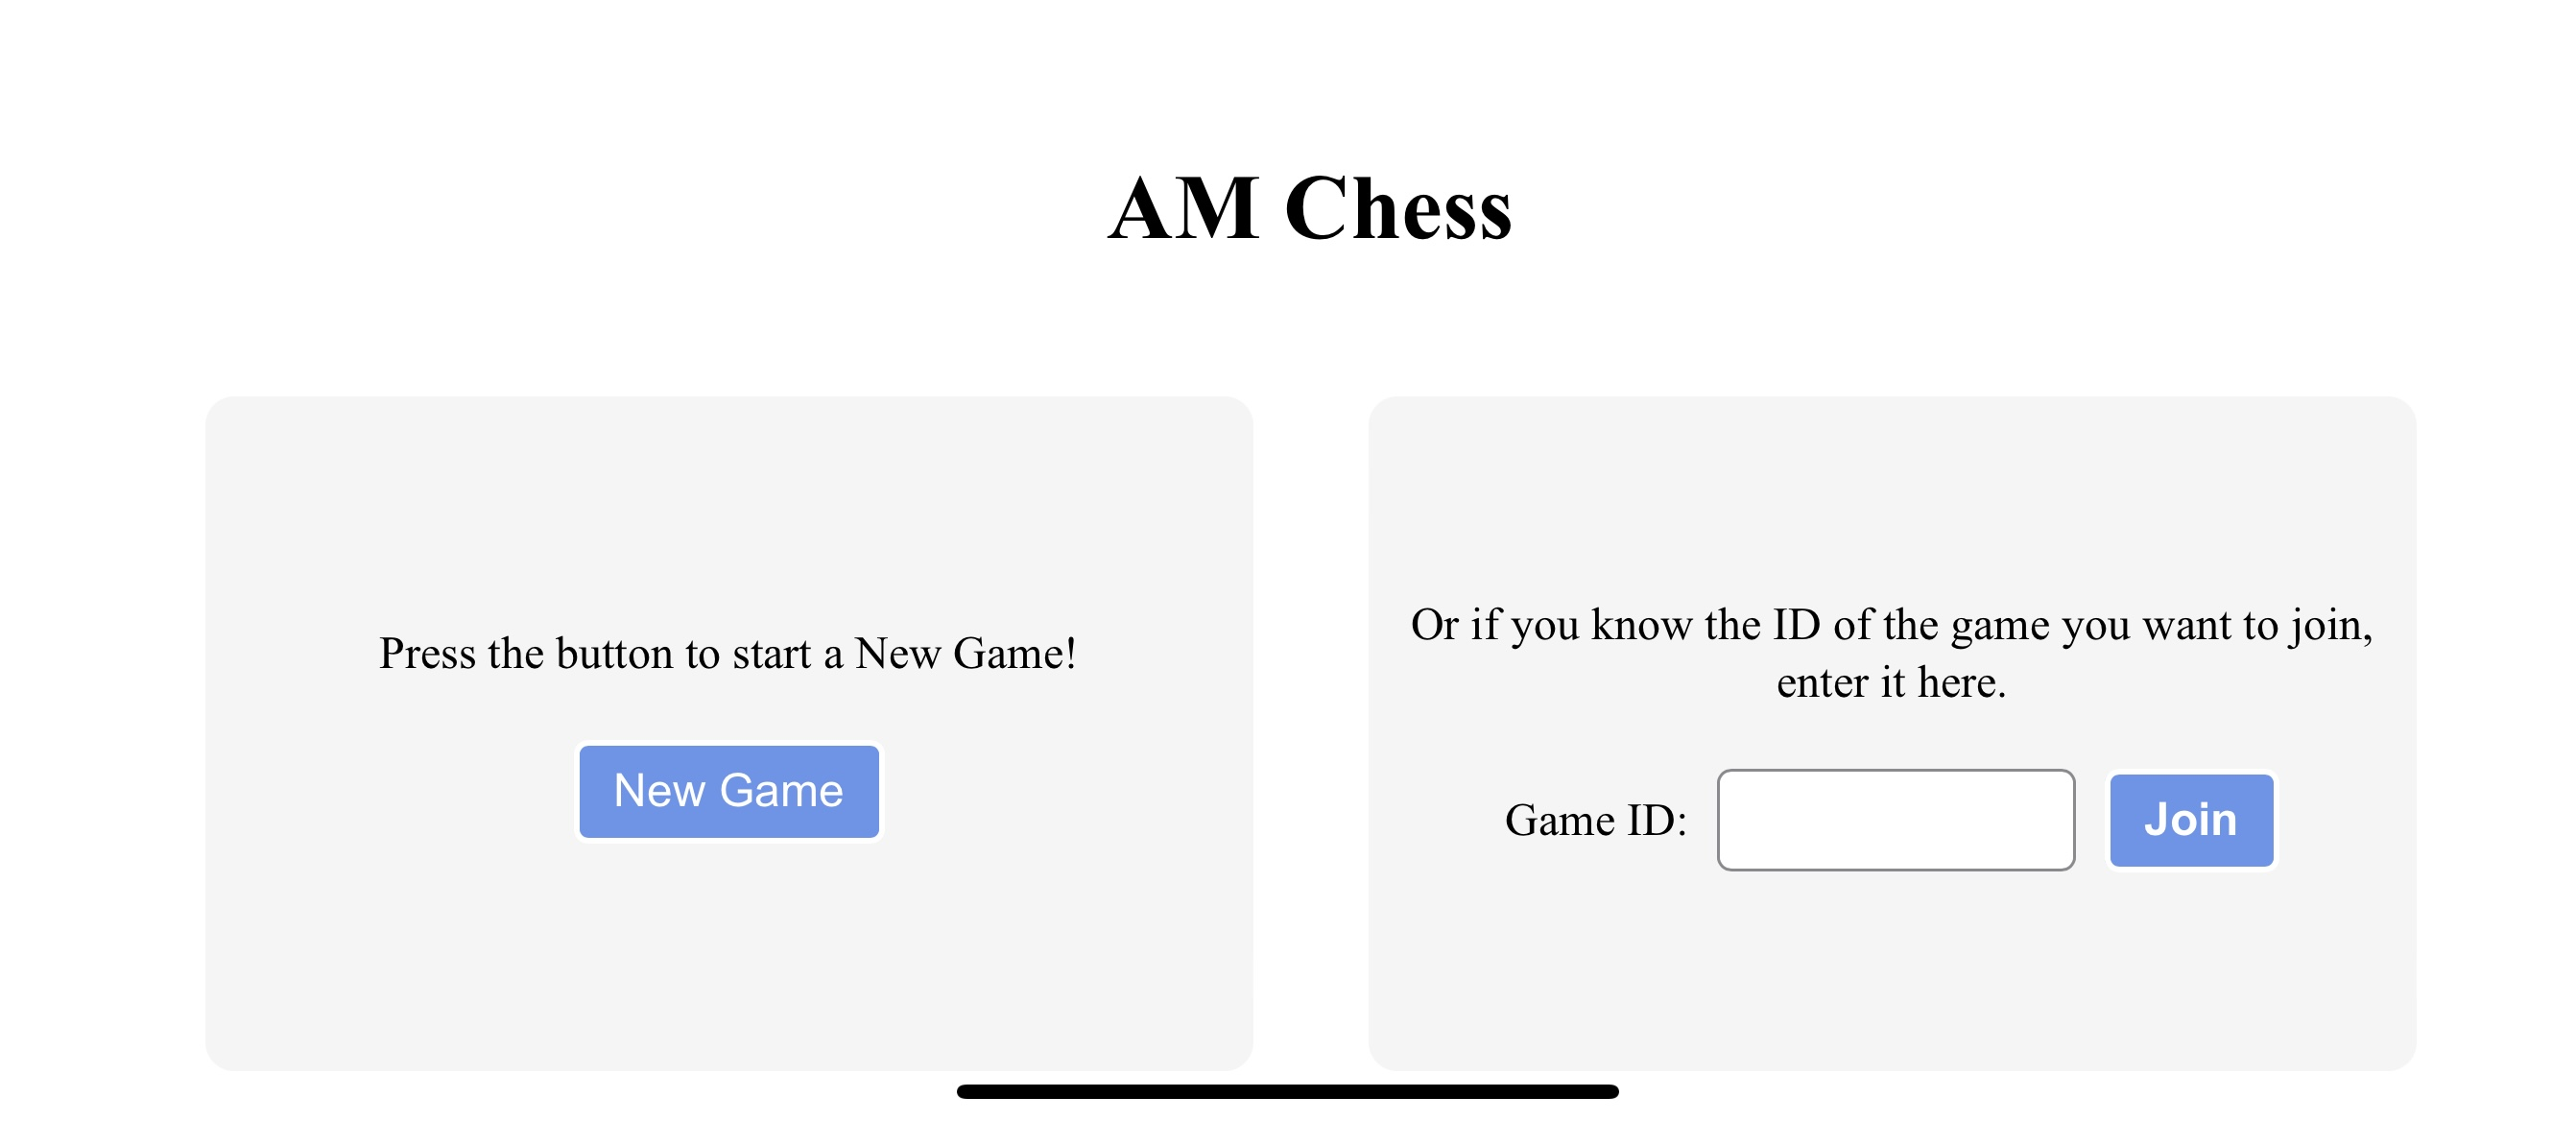
\includegraphics[width=0.6\textwidth]{welcomeHorisontal}}}
        \caption{The welcome page, as seen on a mobile device in both vertical and horisontal orientations respectively}
        \label{fig:responsiveDesign}
    \end{center}
\end{figure}

The benefits of responsive design can also be seen on the chess page. Specifically on computers, if a user resizes the window, the board also changes size. The board will never grow larger than the width and height of its container, so its size is always the minimum of these values. Due to the way that the drawing has been implemented, when resizing the board, the whole thing is drawn again and this requires knowing what pieces are to be drawn on top. Therefore the server is queried every time the window resizes, this includes the duration of dragging the window. This is of course not very efficient and so we can implement a method called debouncing \cite{Debouncing} to reduce the number of times this resize request is made to the server. Debouncing works by setting a timer with a callback to the function you want, in our case requesting the pieces on the board and redrawing the board. However if the the event is called again before the timer has finished, the timer is reset to 0 ticks. Therefore the resize event is only called when the user has finally stop adjusting the size of the window for a period of time.